\documentclass{beamer}

\mode<presentation>
{
  \usetheme{default}
  \usecolortheme{default}
  \usefonttheme{default}
  \setbeamertemplate{navigation symbols}{}
  \setbeamertemplate{caption}[numbered]
  \setbeamertemplate{footline}[page number]
  \setbeamercolor{frametitle}{fg=white}
  \setbeamercolor{footline}{fg=black}
} 

\usepackage[english]{babel}
\usepackage[utf8x]{inputenc}
\usepackage{tikz}
\usepackage{listings}
\usepackage{courier}
\usepackage{array}
\usepackage{bold-extra}
\usepackage{minted}

\xdefinecolor{darkblue}{rgb}{0.1,0.1,0.7}
\xdefinecolor{darkgreen}{rgb}{0,0.5,0}
\xdefinecolor{darkgrey}{rgb}{0.35,0.35,0.35}
\xdefinecolor{darkorange}{rgb}{0.8,0.5,0}
\xdefinecolor{darkred}{rgb}{0.7,0,0}
\xdefinecolor{dianablue}{rgb}{0.18,0.24,0.31}
\definecolor{commentgreen}{rgb}{0,0.6,0}
\definecolor{stringmauve}{rgb}{0.58,0,0.82}

\lstset{ %
  backgroundcolor=\color{white},      % choose the background color
  basicstyle=\ttfamily\small,         % size of fonts used for the code
  breaklines=true,                    % automatic line breaking only at whitespace
  captionpos=b,                       % sets the caption-position to bottom
  commentstyle=\color{commentgreen},  % comment style
  escapeinside={\%*}{*)},             % if you want to add LaTeX within your code
  keywordstyle=\color{blue},          % keyword style
  stringstyle=\color{stringmauve},    % string literal style
  showstringspaces=false,
  showlines=true
}

\lstdefinelanguage{scala}{
  morekeywords={abstract,case,catch,class,def,%
    do,else,extends,false,final,finally,%
    for,if,implicit,import,match,mixin,%
    new,null,object,override,package,%
    private,protected,requires,return,sealed,%
    super,this,throw,trait,true,try,%
    type,val,var,while,with,yield},
  otherkeywords={=>,<-,<\%,<:,>:,\#,@},
  sensitive=true,
  morecomment=[l]{//},
  morecomment=[n]{/*}{*/},
  morestring=[b]",
  morestring=[b]',
  morestring=[b]"""
}

\title[2017-02-08-rootio-femtocode]{Executing code on columnar data: the translation problem and formats that help}
\author{Jim Pivarski}
\institute{Princeton -- DIANA}
\date{February 8, 2017}

\begin{document}

\logo{\pgfputat{\pgfxy(0.11, 8)}{\pgfbox[right,base]{\tikz{\filldraw[fill=dianablue, draw=none] (0 cm, 0 cm) rectangle (50 cm, 1 cm);}}}\pgfputat{\pgfxy(0.11, -0.6)}{\pgfbox[right,base]{\tikz{\filldraw[fill=dianablue, draw=none] (0 cm, 0 cm) rectangle (50 cm, 1 cm);}\includegraphics[height=0.99 cm]{diana-hep-logo.png}\tikz{\filldraw[fill=dianablue, draw=none] (0 cm, 0 cm) rectangle (4.9 cm, 1 cm);}}}}

\begin{frame}
  \titlepage
\end{frame}

\logo{\pgfputat{\pgfxy(0.11, 8)}{\pgfbox[right,base]{\tikz{\filldraw[fill=dianablue, draw=none] (0 cm, 0 cm) rectangle (50 cm, 1 cm);}\includegraphics[height=1 cm]{diana-hep-logo.png}}}}

% Uncomment these lines for an automatically generated outline.
%\begin{frame}{Outline}
%  \tableofcontents
%\end{frame}

%%%%%%%%%%%%%%%%%%%%%%%%%%%%%%%%%%%%%%%%%%%%%%%%%%%%%%%

%% \begin{frame}{Why I'm interested in columnar data}
%% \vspace{0.5 cm}
%% I'm working on a query language and database server to aggregate large samples of HEP data on the fly.

%% \vspace{0.3 cm}
%% \textcolor{darkblue}{Purpose:} to eliminate the need for private skims in most situations.

%% \vfill
%% \begin{center}
%% \large \textcolor{darkblue}{to replace}

%% \vspace{0.3 cm}
%% \includegraphics[width=0.9\linewidth]{workflow.png}
%% \end{center}

%% \vfill
%% \begin{center}
%% \large \textcolor{darkblue}{with}

%% \vspace{0.3 cm}
%% 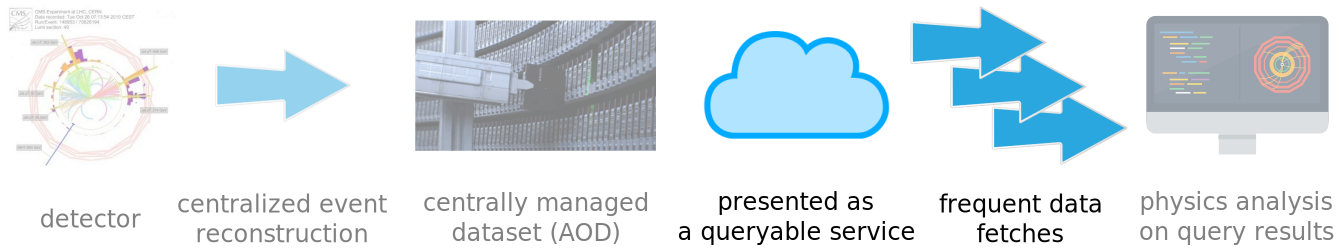
\includegraphics[width=0.9\linewidth]{workflow2.png}
%% \end{center}
%% \end{frame}

%% \begin{frame}{Why I'm interested in columnar data}
%% The query language, Femtocode, plays a similar \mbox{role as TTreeFormula:\hspace{-1 cm}}
%% \begin{itemize}
%% \item a high-level language for the physicist
%% \item usually for filling a histogram (so query responses are small)
%% \item but generally useful for transforming one dataset into another.
%% \end{itemize}

%% \vspace{0.3 cm}
%% However, it's a full-fledged language with assignments and user-defined functions, so that it can encompass a larger part of the analysis.

%% \vspace{0.3 cm}
%% \textcolor{darkgray}{(I've examined SQL, LINQ, and others, and they are not sufficient. I would use a standard if I could.)}
%% \end{frame}

%% \begin{frame}{Why I'm interested in columnar data}
%% The essential feature of Femtocode is that it can transform complex structure-manipulations, which would ordinarily have to be performed in object-oriented code, into a series of vectorized kernels.

%% \vspace{0.3 cm}
%% It operates on columns.
%% \end{frame}

%% \begin{frame}[fragile]{Data reduction without objects}
%% \vspace{0.3 cm}
%% \hspace{-0.25 cm}\textcolor{darkblue}{Example:}
%% \small
%% \begin{minted}{python}
%%   hist = dataset..bin(100, 0, 50, """
%%       muons.map(m => sqrt(m.px**2 + m.py**2)).max()
%%   """)
%% \end{minted}
%% \normalsize

%% \vfill
%% \mbox{\hspace{0.25 cm}\begin{columns}[t]
%% \column{0.5\linewidth}
%% \textcolor{darkblue}{transforms to}
%% \begin{enumerate}
%% \item Pass over all muons, computing $\sqrt{{p_x}^2 + {p_y}^2}$ on all muons, ignoring event boundaries.
%% \item Find the maximum such value for each event.
%% \item Bin those events and fill the histogram.
%% \end{enumerate}

%% \column{0.5\linewidth}
%% \normalsize
%% \textcolor{darkblue}{rather than}
%% \begin{enumerate}
%% \item Loop over events:
%% \begin{enumerate}
%% \item Loop over muons:
%% \begin{enumerate}
%% \item Compute $\sqrt{{p_x}^2 + {p_y}^2}$ for each.
%% \end{enumerate}
%% \item Fill a histogram with the maximum.
%% \end{enumerate}
%% \end{enumerate}
%% \end{columns}}
%% \end{frame}

\begin{frame}{Scope of computability}
\vspace{0.5 cm}
\textcolor{darkblue}{Three types of data transformations:}
\begin{description}
\item[Flat:] apply $N$-argument function to each element of $N$ aligned arrays.

\vspace{0.2 cm}
Known in the Numpy community as a ``ufunc.''

\item[Explode:] emulate (nested) for loops by replicating data in one array so that it becomes aligned with another array.

\item[Reduce:] emulate reducer functions (sum, mean, max\ldots) by combining elements of an array so that it becomes aligned with an outer level of structure.
\end{description}

\vfill
\begin{uncoverenv}<2->
\textcolor{darkblue}{What's missing?}

\vspace{0.2 cm}
``Repeat until convergence.'' Whatever determines ``convergence'' may be different for each element of the array: they'd all wait for the last one, anyway.
\end{uncoverenv}
\end{frame}

\begin{frame}[fragile]{Flat transformations}
\scriptsize
\begin{minted}{python}
import ctypes
import numpy
import numba

libMathCore = ctypes.cdll.LoadLibrary("libMathCore.so")

ChisquareQuantile_ctypes = libMathCore._ZN5TMath17ChisquareQuantileEdd
ChisquareQuantile_ctypes.argtypes = (ctypes.c_double, ctypes.c_double)
ChisquareQuantile_ctypes.restype = ctypes.c_double

@numba.vectorize(["f8(f8, f8)"], nopython=True)
def ChisquareQuantile_Numpy(p, ndf):
    return ChisquareQuantile_ctypes(p, ndf)

p = numpy.random.uniform(0, 1, int(1e6))

result = [ChisquareQuantile_ctypes(pi, 100) for pi in p]
# 10.30 seconds

result = ChisquareQuantile_Numpy(p, 100)
# 3.22 seconds
\end{minted}
\end{frame}



\end{document}
